
%(BEGIN_QUESTION)
% Copyright 2006, Tony R. Kuphaldt, released under the Creative Commons Attribution License (v 1.0)
% This means you may do almost anything with this work of mine, so long as you give me proper credit

\vbox{\hrule \hbox{\strut \vrule{} $\int f(x) \> dx$ \hskip 5pt {\sl Calculus alert!} \vrule} \hrule}

Tenk deg at vi måler kommunal vannstrøm gjennom et rør ved hjelp av en turbinmåler:

$$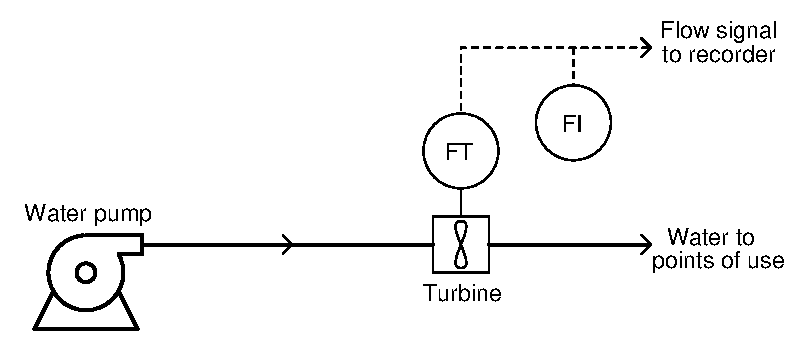
\includegraphics[width=15.5cm]{i00543x01.eps}$$

Anta at ledelsen i kommunen ønsker en løpende total av vann{\it volum} i tillegg til vannstrøm. Med andre ord vil de ha en teller som summerer antall gallon som har passert gjennom måleren. En operatør registrerer totalvolumet ved slutten av hver dag og nullstiller telleren for neste døgn.

To instrumentteknikere har ulike forslag til hvordan dette kan gjøres. Den ene teknikeren mener det er enkelt å {\it integrere} 4--20 mA-strømningssignalet elektronisk for å få et volumsignal, mens den andre foreslår å hente signal direkte fra turbinens ``pick-up'' i stedet for 4--20 mA-signalet, og sende pulssignalet til en digital teller.

Utdyp disse to planene, og begrunn deretter hvilket forslag du selv ville valgt, eventuelt et helt annet.

\underbar{file i00543}
%(END_QUESTION)





%(BEGIN_ANSWER)

Kalkulusoperasjonen {\it tidsintegrasjon} ``opphever'' matematisk derivasjon. Hvis vi vet at strømning bare er endringshastigheten til volum med hensyn på tid, bør en integratorkrets kunne oppheve strømningssignalet og gi et volumsignal:

$$Q = {dV \over dt} \hbox{\hskip 30pt Strømning er tidsderivert av volum}$$

$$V = \int^T_0 Q \> dt \hbox{\hskip 30pt Volum er tidsintegralet av strømning}$$

En enkel analog krets for å utføre tidsintegrasjon ser slik ut:

$$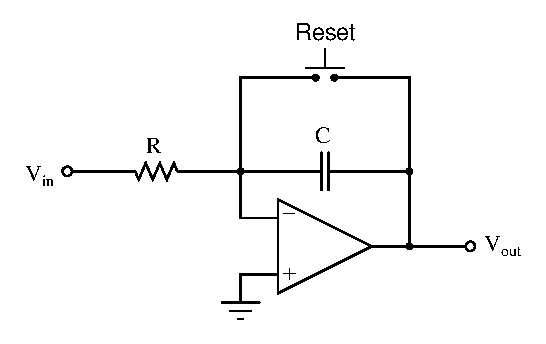
\includegraphics[width=15.5cm]{i00543x02.eps}$$

$$V_{out} = - {1 \over {RC}} \int^T_0 V_{in} \> dt$$

Vi måtte selvsagt lagt til en del ekstra komponenter for å gjøre kretsen klar til å ta imot et 4--20 mA-signal. Det bør også nevnes at integrasjon over lange tidsperioder nesten alltid gjøres digitalt på grunn av driftsproblemer i analoge kretser.

\vskip 10pt

Den andre teknikerens idé -- å klokke en digital teller fra turbinmålerens pulsutgang -- vil være enklere (mindre krets) og mer praktisk (mindre å kalibrere).

%(END_ANSWER)





%(BEGIN_NOTES)


%INDEX% Måling, strømning: totalisator

%(END_NOTES)

